\documentclass[12pt,a4paper]{article}
\usepackage[utf8]{vietnam}
\usepackage{amsmath,amssymb}
\usepackage{tabularx}
\usepackage{tikz}
\usetikzlibrary{calc,angles,quotes,arrows.meta,patterns}
\usepackage{xcolor}
\usepackage{enumitem}
\usepackage{fancyhdr}
\usepackage{graphicx}
\usepackage[top=0.9cm, bottom=0.9cm, left=1.2cm, right=1.2cm]{geometry}
\usepackage[dethi]{ex_test}
\SAOPTN{widthSA=3.2,heightSA=0.62}

\setlength{\headheight}{15pt}
\setlength{\parskip}{0pt}

\pagestyle{fancy}
\fancyhf{}
\rhead{\textit{Môn Toán 9 -- Đề số 07}}
\lhead{\textit{Bộ đề ôn tập Giữa học kì I}}
\cfoot{\thepage}

\begin{document}

% --- KHUNG TIÊU ĐỀ ĐỀ THI ---
\noindent
\begin{tabularx}{\linewidth}{X r}
\textbf{TRƯỜNG THCS: \dotfill} & \textbf{ĐỀ KIỂM TRA ĐỊNH KỲ GIỮA HỌC KỲ I} \\
\textbf{Họ và tên: \dotfill} & \textbf{NĂM HỌC 2026 -- 2027} \\
\textbf{Lớp: \dotfill \quad SBD: \dotfill} & \textbf{Môn: TOÁN 9} \\
\hline
\end{tabularx}
\vspace{2mm}

\begin{center}
  \textbf{\large ĐỀ ÔN TẬP GIỮA HỌC KỲ I -- ĐỀ SỐ 07}\\
  \textit{Thời gian làm bài: 90 phút (Không kể thời gian phát đề)}
\end{center}
\vspace{1mm}

% --- PHẦN I ---
\noindent\textbf{\large PHẦN I. CÂU TRẮC NGHIỆM NHIỀU PHƯƠNG ÁN LỰA CHỌN (3,0 điểm)}

\textit{Thí sinh trả lời từ câu 1 đến câu 12. Mỗi câu hỏi thí sinh chỉ chọn một phương án duy nhất.}

\vspace{1mm}
\begin{ex}
Phương trình nào sau đây là phương trình bậc nhất hai ẩn?
\choice
{\True $-x - y = 0$}
{$x^2 - 2y + 1 = 0$}
{$\frac{1}{x} + \frac{1}{y} = \frac{1}{2}$}
{$x + 2xy - y = 1$}
\end{ex}

\begin{ex}
Phương trình $0x + 5y = 10$ có nghiệm tổng quát là:
\choice
{\True $(x; 2)$ với $x \in \mathbb{R}$}
{$(2; y)$ với $y \in \mathbb{R}$}
{$(x; 0)$ với $x \in \mathbb{R}$}
{$(0; y)$ với $y \in \mathbb{R}$}
\end{ex}

\begin{ex}
Cặp số nào sau đây là nghiệm của hệ phương trình $\begin{cases} 2x + y = 3 \\ y = 1 \end{cases}$?
\choice
{$(2; 1)$}
{$(2; -1)$}
{$(1; -1)$}
{\True $(1; 1)$}
\end{ex}

\begin{ex}
Trong các hệ phương trình bậc nhất hai ẩn sau, hệ phương trình nào nhận cặp số $(-1; 3)$ làm nghiệm?
\choice
{$\begin{cases} 2x + y = 1 \\ -x - y = 2 \end{cases}$}
{$\begin{cases} 3x + y = 8 \\ -x + y = 5 \end{cases}$}
{\True $\begin{cases} x + y = 2 \\ 3x - y = -6 \end{cases}$}
{$\begin{cases} 2x - y = 5 \\ 4x + 2y = 2 \end{cases}$}
\end{ex}

\begin{ex}
Biết rằng hệ phương trình $\begin{cases} 5x - y = 8 \\ 3x - ay = 1 \end{cases}$ có nghiệm $(2; 2)$. Giá trị của $a$ là:
\choice
{$a = -\frac{1}{2}$}
{\True $a = \frac{5}{2}$}
{$a = 1$}
{$a = -2$}
\end{ex}

\begin{ex}
Phương trình $(x - 7)(x + 2) = 0$ có nghiệm là:
\choice
{$x = 7; x = 2$}
{\True $x = 7; x = -2$}
{$x = -7; x = 2$}
{$x = -7; x = -2$}
\end{ex}

\begin{ex}
Cho tam giác $MNP$ vuông tại $N$. Hệ thức nào sau đây là đúng?
\choice
{\True $MN = MP \cdot \sin P$}
{$MN = MP \cdot \cos P$}
{$MN = MP \cdot \tan P$}
{$MN = MP \cdot \cot P$}
\end{ex}

\begin{ex}
Cho đường tròn $(O)$ có hai bán kính $OA, OB$ tạo thành góc ở tâm $\widehat{AOB} = 60^\circ$. Điểm $n$ nằm trên cung nhỏ $AB$, điểm $m$ nằm trên cung lớn $AB$. Số đo các cung $AnB$ và $AmB$ lần lượt là:
\begin{center}
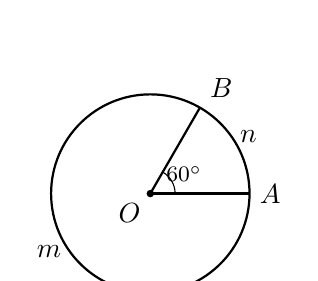
\begin{tikzpicture}[scale=0.9]
  \coordinate (O) at (0,0);
  \draw[thick] (O) circle (1.4);
  \coordinate (A) at (1.4,0);
  \coordinate (B) at (60:1.4);
  \draw[thick] (O) -- (A) node[right]{$A$};
  \draw[thick] (O) -- (B) node[above right]{$B$};
  \fill (O) circle (1.5pt) node[below left]{$O$};
  \draw (0.35,0) arc (0:60:0.35);
  \node at (30:0.55) {\footnotesize $60^\circ$};
  \node at (30:1.6) {$n$};
  \node at (210:1.65) {$m$};
\end{tikzpicture}
\end{center}
\choice
{$120^\circ$ và $300^\circ$}
{$60^\circ$ và $60^\circ$}
{\True $60^\circ$ và $300^\circ$}
{$60^\circ$ và $120^\circ$}
\end{ex}

\begin{ex}
Một cột đèn có bóng trên mặt đất dài $7{,}2\text{ m}$. Các tia nắng mặt trời tạo với mặt đất một góc xấp xỉ $42^\circ$. Chiều cao xấp xỉ của cột đèn là:
\begin{center}
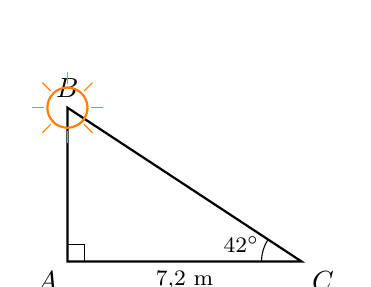
\begin{tikzpicture}[scale=0.85]
  \coordinate (A) at (0,0);
  \coordinate (B) at (0,2.3);
  \coordinate (C) at (3.5,0);
  \draw[thick] (A) -- (B) node[above]{$B$} -- (C) node[below right]{$C$} -- cycle;
  \node[below left] at (A) {$A$};
  \draw (A) ++(0,0.25) -- ++(0.25,0) -- ++(0,-0.25);
  \draw (C) ++(-0.6,0) arc (180:146:0.6);
  \node at (2.6,0.25) {\footnotesize $42^\circ$};
  \node[below] at (1.75,0) {\footnotesize $7{,}2\text{ m}$};
  \draw[orange, thick] (B) circle (0.3);
  \foreach \ang in {0, 45, 90, 135, 180, 225, 270, 315} {
    \draw[orange, thin] (B) ++(\ang:0.35) -- ++(\ang:0.18);
  }
\end{tikzpicture}
\end{center}
\choice
{\True $6{,}48\text{ m}$}
{$8\text{ m}$}
{$4{,}82\text{ m}$}
{$5{,}35\text{ m}$}
\end{ex}

\begin{ex}
Kết quả rút gọn của biểu thức $\sqrt[3]{8} + \sqrt[3]{-27} + \sqrt[3]{-64}$ là:
\choice
{$5$}
{\True $-5$}
{$9$}
{$-9$}
\end{ex}

\begin{ex}
Cho tam giác $MNE$ vuông tại $M$, đường cao $MH$. Hệ thức nào sau đây là đúng?
\choice
{\True $\frac{1}{MH^2} = \frac{1}{MN^2} + \frac{1}{ME^2}$}
{$MH^2 = MN^2 + ME^2$}
{$\frac{1}{MH} = \frac{1}{MN} + \frac{1}{ME}$}
{$MH^2 = NE \cdot HE$}
\end{ex}

\begin{ex}
Cho tam giác $ABC$ vuông tại $A$, đường cao $AH$, có $AB = 12\text{ cm}, BC = 20\text{ cm}$. Độ dài $BH, CH$ lần lượt là:
\choice
{$BH = 7{,}2\text{ cm}; CH = 11{,}8\text{ cm}$}
{$BH = 9{,}2\text{ cm}; CH = 10{,}8\text{ cm}$}
{\True $BH = 7{,}2\text{ cm}; CH = 12{,}8\text{ cm}$}
{$BH = 7{,}2\text{ cm}; CH = 12\text{ cm}$}
\end{ex}


\vspace{1mm}
\noindent\textbf{BẢNG TRẢ LỜI TRẮC NGHIỆM PHẦN I:}
\begin{center}
\begin{tabular}{|c|c|c|c|c|c|c|c|c|c|c|c|c|}
\hline
\textbf{Câu} & \textbf{1} & \textbf{2} & \textbf{3} & \textbf{4} & \textbf{5} & \textbf{6} & \textbf{7} & \textbf{8} & \textbf{9} & \textbf{10} & \textbf{11} & \textbf{12} \\
\hline
\textbf{Chọn} & \rule{0pt}{0.65cm} & & & & & & & & & & & \\
\hline
\end{tabular}
\end{center}
\vspace{2mm}

% --- PHẦN II ---
\noindent\textbf{\large PHẦN II. CÂU TRẮC NGHIỆM ĐÚNG SAI (2,0 điểm)}

\textit{Thí sinh trả lời từ câu 1 đến câu 2. Trong mỗi ý a), b), c), d) ở mỗi câu, thí sinh chọn đúng hoặc sai.}

\vspace{1mm}
\begin{ex}
Cho bất đẳng thức $a > b$. Xét tính Đúng/Sai của các khẳng định sau:
\choiceTF
{\True $a - 4 > b - 4$.}
{$-3a > -3b$.}
{\True $-2a + 3 < -2b + 3$.}
{\True $5a - 1 > 5b - 2$.}
\end{ex}

\begin{ex}
Cho tam giác $ABC$ vuông tại $A$, đường cao $AH$. Biết $AC = 6\text{ cm}, BC = 10\text{ cm}$. Xét tính Đúng/Sai của các khẳng định sau:
\choiceTF
{\True $\sin B = \frac{3}{5}$.}
{$\tan C = \frac{3}{4}$.}
{\True $AH = 4{,}8\text{ cm}$.}
{Chu vi của tam giác $ABH$ bằng $14{,}4\text{ cm}$.}
\end{ex}


\vspace{1mm}
\noindent\textbf{BẢNG TRẢ LỜI ĐÚNG SAI PHẦN II:}
\begin{center}
\begin{tabular}{|c|c|c|c|c||c|c|c|c|c|}
\hline
\textbf{Câu} & \textbf{Lệnh hỏi} & \textbf{Đúng} & \textbf{Sai} & \textbf{Điểm} & \textbf{Câu} & \textbf{Lệnh hỏi} & \textbf{Đúng} & \textbf{Sai} & \textbf{Điểm} \\
\hline
 & a) & & & & & a) & & & \\
\cline{2-4}\cline{7-9}
\textbf{1} & b) & & & & \textbf{2} & b) & & & \\
\cline{2-4}\cline{7-9}
 & c) & & & & & c) & & & \\
\cline{2-4}\cline{7-9}
 & d) & & & & & d) & & & \\
\hline
\end{tabular}
\end{center}
\vspace{2mm}

% --- PHẦN III ---
\noindent\textbf{\large PHẦN III. CÂU TRẮC NGHIỆM TRẢ LỜI NGẮN (1,0 điểm)}

\textit{Thí sinh trả lời từ câu 1 đến câu 2. Viết câu trả lời vào ô quy định.}

\vspace{1mm}
\begin{ex}
Trong các phương trình sau:\par (1) $3\sqrt{y} - 2x = 0$; \quad (2) $2x + y = 0$; \quad (3) $x^2 - y^2 = 12$; \quad (4) $2x + y + 3z = 0$.\par Phương trình bậc nhất hai ẩn là phương trình số mấy?
\shortans{Phương trình (2)}
\end{ex}

\begin{ex}
Cho tam giác $ABC$ vuông tại $A$, biết $AB = 12\text{ cm}, AC = 9\text{ cm}, BC = 15\text{ cm}$. Tính số đo góc $B$ (làm tròn đến độ).
\shortans{$37^\circ$}
\end{ex}


\vspace{2mm}
% --- PHẦN IV ---
\noindent\textbf{\large PHẦN IV. TỰ LUẬN (4,0 điểm)}

\textit{Thí sinh trình bày chi tiết lời giải vào giấy làm bài.}

\vspace{1mm}
\noindent\textbf{Câu 1 (2,0 điểm).}

Giải các phương trình và hệ phương trình sau:\par a) $(4x + 5)(3x - 2) = 0$.\par b) $\frac{4}{x(x - 1)} + \frac{3}{x} = \frac{4}{x - 1}$.\par c) $\begin{cases} x - 3y = 4 \\ -2x + 6y = -8. \end{cases}$

\vspace{2mm}
\noindent\textbf{Câu 2 (1,5 điểm).}

Người ta cho thêm $1\text{ kg}$ nước vào dung dịch $A$ (chứa axit $X$) thì được dung dịch $B$ có nồng độ axit là $20\%$. Sau đó lại cho thêm $1\text{ kg}$ axit $X$ vào dung dịch $B$ thì được dung dịch $C$ có nồng độ axit là $33\frac{1}{3}\%$. Tính nồng độ axit của dung dịch $A$ ban đầu.

\vspace{2mm}
\noindent\textbf{Câu 3 (1,0 điểm).}

Một cầu trượt trong công viên có độ dốc là $28^\circ$ và có độ cao là $2{,}1\text{ m}$. Tính độ dài của mặt cầu trượt (làm tròn đến chữ số thập phân thứ nhất).
\begin{center}
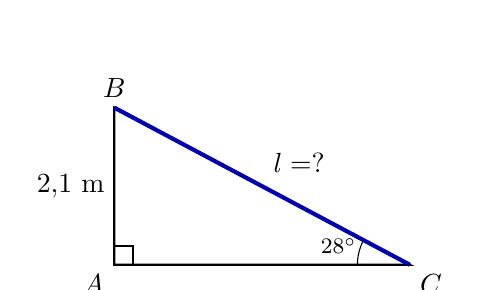
\begin{tikzpicture}[scale=0.95]
  \coordinate (A) at (0,0);
  \coordinate (B) at (0,2.1);
  \coordinate (C) at (3.95,0);
  \draw[thick] (A) node[below left]{$A$} -- (B) node[above]{$B$} -- (C) node[below right]{$C$} -- cycle;
  \draw (A) ++(0,0.25) -- ++(0.25,0) -- ++(0,-0.25);
  \draw (C) ++(-0.7,0) arc (180:152:0.7);
  \node at (3.0,0.25) {\footnotesize $28^\circ$};
  \node[left] at (0,1.05) {$2{,}1\text{ m}$};
  \node[above right] at (2.0,1.1) {$l = ?$};
  \draw[line width=1.5pt, blue!70!black] (B) -- (C);
\end{tikzpicture}
\end{center}

\vspace{2mm}
\noindent\textbf{Câu 4 (0,5 điểm).}

Cho tam giác $ABC$ vuông tại $A$. Chứng minh rằng $\sin^2 B + \sin^2 C = 1$.

\vspace{2mm}

\vfill
\begin{center}
  \textbf{--- HẾT ---}
\end{center}
\end{document}
